\chapter{Mathematical Background}

Frequently multi-agent systems are modeled as a distributed optimization problem. Each agent looks for an optimal solution to a specific task, and it could solve it with the cooperation of its neighbors or without it. Indeed, it is essential to design and implement strategies to manage communication and control the interconnect network optimally. This chapter presents a brief explanation of different techniques used for this purpose. Some relate to modeling, analyzing, and managing the entire network of agents. The control and communications techniques are shown in-depth in chapter \ref{controller_architecture}. 
\\

% -----------------------------------------------------------------

\section{Graph Theory}
\label{sec:game_theory}



A graph is defined as a mathematical and graphical representation of a network. Some of the most common uses of graph representation are people's social interaction in social networks, interconnected networks of robots, servers connected to the internet, cellphones connected to the telephone service, and much more, Fig.  \ref{fig:Social_net}.


\begin{figure}[h]
\begin{center}
    
\includegraphics[width=0.3\textwidth]{Kap2/Network.png}
    \caption{Social Network.}
    \label{fig:Social_net}
\end{center}
\end{figure}


% An edge or link represents multiple kinds of relations, depending on the application, e.g., the local position in a network of vehicles in a speedway or transactions between an exchange bank network. Two vertices (vi, vj) are adjacent if exist an edge eij=(i,j)E  between vi and vj. the neighbors of i is denotes by the set N_i

A graph $\mathcal{G} = (\mathcal{V,E,W})$ consists of the joint of three fundamental parts. A set of vertices (or nodes) $\mathcal{V} = \left\{ v_o,v_1, ... v_n \right\}$, A set of edges (or links) $\mathcal{E} \subseteq  \mathcal{V} \times  \mathcal{V} =  \left \{ e_{1,2},e_{2,3},...,e_{i,j} \right \}$ and a weight matrix $\matchal{W}$ defined as:\\

\begin{equation}
\mathcal{W}  = \mathcal{W}_{i,j} \left\{ \begin{array}{cl}
> 0 & if (i;j) \in \mathcal{E}, \\
=0 & if (i;j) \notin  \mathcal{E}.
\end{array} \right.
\end{equation}


\begin{figure}[h]
\begin{center}
    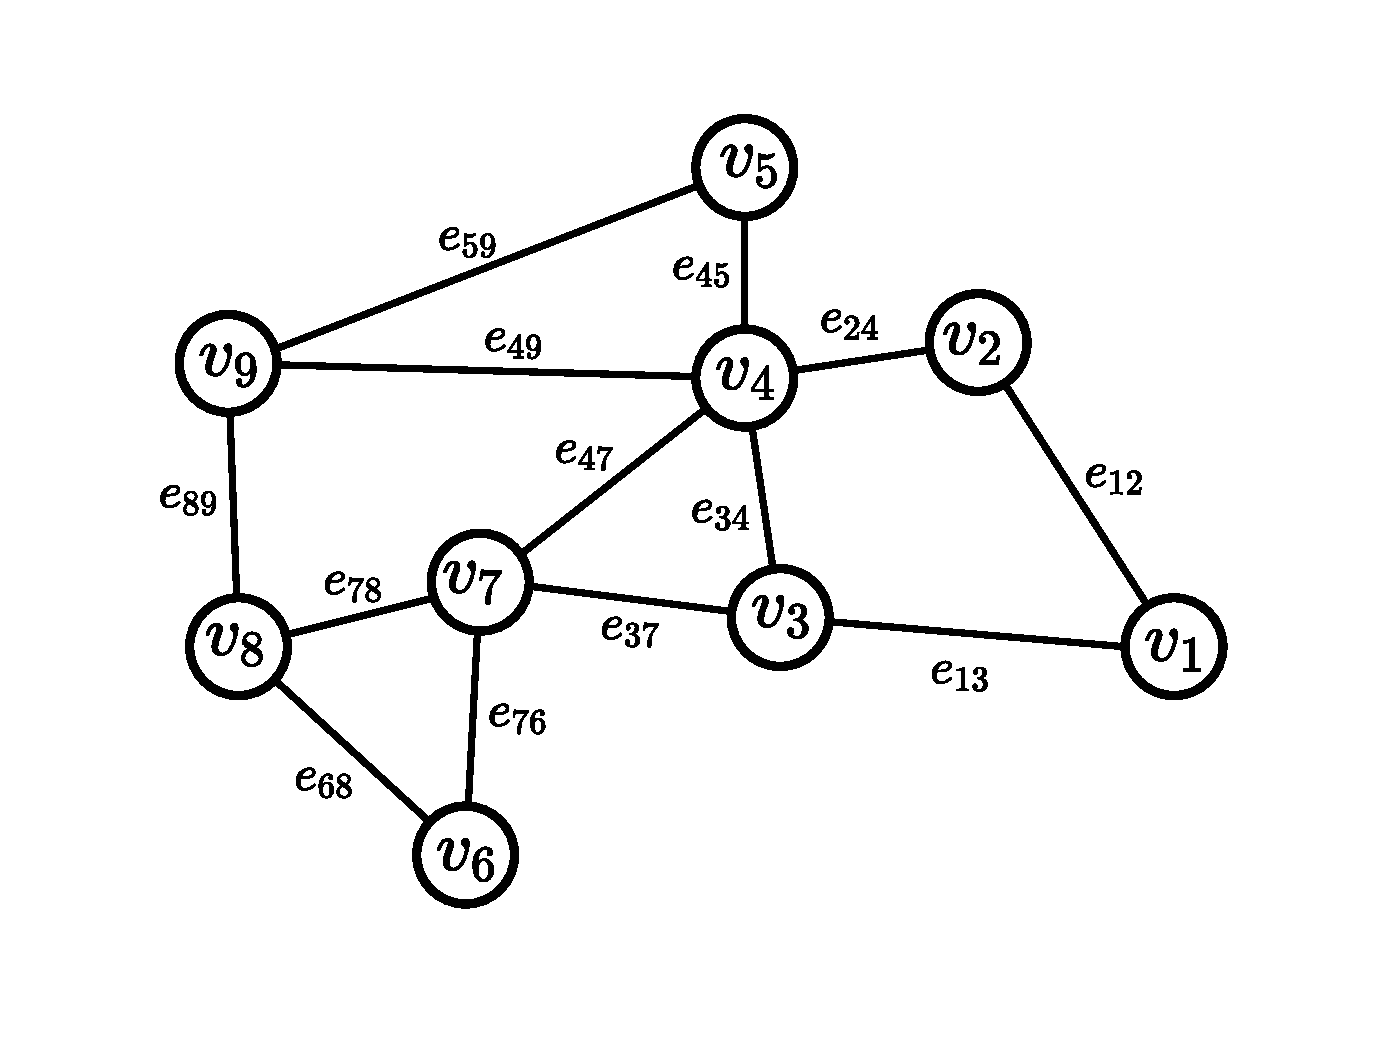
\includegraphics[width=0.6\textwidth]{Kap2/Graph-01.eps}
    \caption{ Graph of Network system.}
    \label{fig:Graph}
\end{center}
\end{figure}


A set of vertices is a group of agents (or nodes) $v = 1,..., n$, where each node is an information source. It could be auto-generated or retransmitted by other nodes. In Fig \ref{fig:Graph} the set of vertices is $\mathcal{V} = \left\{ v_1,v_2,v_3,v_4,v_5,v_6,v_7,v_8,v_9 \right\}$.
However, the edges (or links) are how the information is shared. It could be directed or undirected depending on how the information is transmitted if just a node can transmit or transmit-receive. In the previous example, the set of edges is $ \mathcal{E} = \left\{ e_{12},e_{13},e_{24},e_{34},e_{37},e_{45},e_{47},e_{49},e_{59},e_{68},e_{76},e_{78},e_{89} \right\}$, and lastly the weight matrix is an algebraic representation of the entire interconnected system. If exist a connection between vertice I and j in the matrix, it will be 1; otherwise, it will be 0. In fig \ref{fig:Graph} the weight matrix is:


\begin{equation*}
\centering
\mathcal{W} = \begin{bmatrix}
0 & 1 & 1 & 0 & 0 & 0 & 0 & 0 & 0 \\
1 & 0 & 0 & 1 & 0 & 0 & 0 & 0 & 0 \\
1 & 0 & 0 & 1 & 0 & 0 & 1 & 0 & 0 \\
0 & 1 & 1 & 0 & 1 & 0 & 1 & 0 & 1 \\
0 & 0 & 0 & 1 & 0 & 0 & 0 & 0 & 1 \\
0 & 0 & 0 & 0 & 0 & 0 & 1 & 1 & 0 \\
0 & 0 & 1 & 1 & 0 & 1 & 0 & 1 & 0 \\
0 & 0 & 0 & 0 & 0 & 1 & 1 & 0 & 1 \\
0 & 0 & 0 & 1 & 1 & 0 & 0 & 1 & 0
\end{bmatrix}
\end{equation*}
\\

The neighborhood of node $v_{i}$ is the set of nodes $\mathcal{N}_{i} \subseteq  \mathcal{V}$ that have a direct interaction with agent $i$. This set of edges could be directed or undirected depending on their communication. A graph $\mathcal{G}$ is connected if a connection exists between two or more nodes and there is a route between all nodes in the set $\mathcal{V}$. Finally, the set of nodes of a graph has a degree;  It depends on the number of neighbors of each node. If all graph nodes have the same degree, the graph is called a regular graph.\\

A graph could be represented as a joint of multiple matrices. These matrices show information about each node with the other. 






% ---------------------------- degreee and adjacency --------------------------
\section*{Degree and Adjacency Matrix}

The degree of a node $v_{i}$ is represented as $d(v_{i})$, which is the name of the cardinality of a node, and it represents the number of agents connected with node $i$. Therefore, The degree matrix is a diagonal matrix with the degree values of each node:

\begin{equation}
    \Delta (\mathcal{G}) = \begin{bmatrix}
d(v_{1}) &   0    &  \cdots & 0\\ 
0      & d(v_{2}) & \cdots &  0 \\ 
\vdots & \vdots   & \ddots  & \vdots\\ 
0      & 0        & \cdots & d(v_{n}) 
  \end{bmatrix}
\end{equation}


In addition, an adjacency matrix exists where the relationship of each node with each other is represented. Moreover, the adjacency matrix is defined as:

\begin{equation}
    \left [ Y(\mathcal{G}) \right ]_{ij} = \left\{\begin{matrix}
1, & \text{if } v_{i}v_{j} \in \mathcal{E},\\ 
0, & \text{Otherwise.} 
\end{matrix}\right.
\end{equation}


\section*{Incidence Matrix}
There are directional or bidirectional graphics on its edges. If there is a graph with directed edges, it is called a digraph $\mathcal{D}$. Therefore, a digraph is described by its incidence matrix, representing the orientation of each edge of the graph. With the previous information, it is possible to analyze factors such as stability, network controllability, communication times, and the sequence that the information follows to reach each agent. The incidence matrix is defined as:

\begin{equation}
    I_{ij}(\mathcal{G}) = \left\{\begin{matrix*}[l]
-1, & \text{if } v_{i} \text{ is the tail of } v_{j},\\ 
1, & \text{if } v_{i} \text{ is the head of } v_{j},\\ 
0, &  \text{Otherwise.   }
\end{matrix*}\right.
\end{equation}

A graph could also have weights in its connections, representing the importance of the neighbour's information on each node. If a graph has weighted edges, it is called a weight graph. Consequently, in a weight graph, the adjacency matrix is built by the following definition:


\begin{equation}
    Ad(\mathcal{G}) = \left\{\begin{matrix}
\omega_{ij},   & \text{if } (v_{i}v_{j}) \in \mathcal{E}, \\ 
0, &  \text{Otherwise.}
\end{matrix}\right.
\end{equation}

% ---------------------------- laplacian ----------------------------
\section*{Laplacian}

The Laplacian of a graph is another fundamental representation of a graph. The way of representing a Laplacian graph of a graph $\mathcal{G}$ is by using the joint of adjacency and degree matrix as follows:

\begin{equation}
    L(\mathcal{G}) = \Delta (\mathcal{G}) - Y\mathcal(G)
\end{equation}

Laplacian matrix must be symmetric if it is a digraph or asymmetric otherwise. 










% representacion matricial de grafos

% matriz de grafo y de adyacencia 



% -----------------------------------------------------------------------------


\section{Model Predictive Control}
Model Predictive Control is a control theory used to manage some variables optimally into a function looking at a specific result. The main idea is to use a discrete model of the entire system to predict future system states. With the capability of predicting future behaviours over a finite-time prediction and control horizon $H_u$ and $H_p$, depending on different inputs. It is possible to optimize the input control to achieve an optimal solution. The process is to apply an optimal input signal to the system and recalc the next optimal step. This process is repetitive, while the system aims at the principal objective \cite{3t_sequential}. 
\\

The first step measures the error of the actual and desired state and the amount of energy implemented, as shown in Fig  \ref{fig:mpc1}. With this information, optimize the states error and control input to achieve its objective Fig \ref{fig:mpc2}. MPC benefits are achieving the main goal while considering some constraints, the ease of design, simulation, and implementation in different systems, and the powerful way to control linear and nonlinear systems. This section describes the mathematical theory of a Model Predictive Control and its applications in the described scenario.


\subsection{Dynamic Prediction Model}

Considering a discrete model system (\ref{eq:mpc2}) and the observably output model (\ref{eq:mpc}), where $x(t) \in \mathbb{R}^n$ represents the state values at time $t$, the $u(t) \in \mathbb{R}^m$ variable as the discrete control input signal at the time $t$. The output is represented as  $y(t) \in \mathbb{R}^p$.

\begin{align}
    x(t+1) = f(x(t),u(t)),\label{eq:mpc2}\\
    y(t) = g(x(t),u(t)). \label{eq:mpc}
\end{align}

The dynamic equation \ref{eq:mpc2} express the evolution  of the states $f:\mathbb{R}^n \times \mathbb{R}^m \to  \mathbb{R}^n$ over the horizon $H_u$ and the output function shows the behavior $g:\mathbb{R}^n \times \mathbb{R}^m \to  \mathbb{R}^p$ over the horizon $H_p$. 
In order to reduce computation load and time delays, a linearized prediction model can be set up using the state evolution in \ref{eq:dynamic}. This thesis document linearized some convex models; however, all dynamic models will be explained in-depth in the next chapter. While the controller works, this linearization is processed in each iteration around the actual states. Hence, a matrix E is added to the state matrix A and input matrix B. Future states are predicted using the following iterative substitution:

\begin{align}
x(t+1) & = Ax(t) + Bu(t)+E \\
x(t+2) & = Ax(t+1) + Bu(t+1)+E\\
       & = A^2x(t) + ABu(t)+AE +Bu(t+1) +E\\
       & \vdots  \\
x(t+H_u) & = A^{H_u}x(t) + A^{H_u-1}Bu(t)+\cdots + Bu(t+H_u-1)+ A^{H_u-1}E+\cdots +E\\
      & \vdots  \\
x(t+H_p) & = A^{H_p}x(t) + A^{H_p-1}Bu(t)+\cdots + Bu(t+H_p-1)+ A^{H_p-1}E+\cdots +E
\label{eq:dynamic}
\end{align}

The resulting system is represented by matrices $A(t) \in \mathbb{R}^{n \times n}, B(t) \in \mathbb{R}^{n \times m}, C(t) \in \mathbb{R}^{p \times n} $ and $E(t) \in \mathbb{R}^{n}$ after linearization. The previous predicted linear model is used when the dynamic model, constraints, and objective function are nonlinear and the computing system has low resources. If this linearization is avoided, the calc could be slower, and the control system could be unstable.


\begin{figure}[H]
\begin{center}
    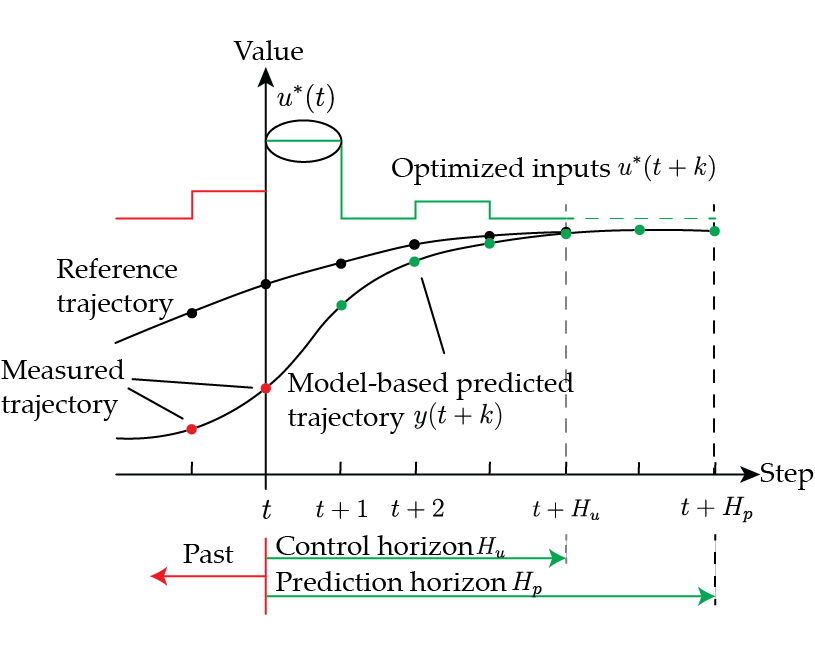
\includegraphics[width=0.6\textwidth]{Kap2/mpc1.png}
    \caption{Control and state signals, First iteration.} 
    \label{fig:mpc1}
\end{center}
\end{figure}

\begin{figure}[H]
\begin{center}
    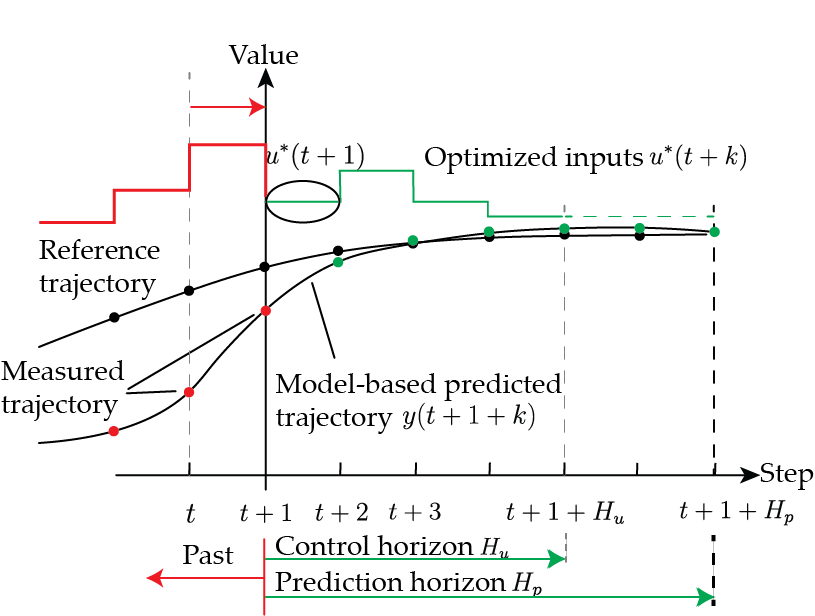
\includegraphics[width=0.6\textwidth]{Kap2/mpc2.png}
    \caption{Control and state signals, Second iteration.}
    \label{fig:mpc2}
\end{center}
\end{figure}




\subsection{Objective Function}

The objective function is the principal function representing the controller's aim that needs to be achieved. This function is also called the cost function. Generally, it is divided into two parts: the \textit{Running cost} and \textit{Terminal costs}. The running cost penalizes the difference between the actual and desired states and control inputs. It allows for tracking a reference and optimizing the consumption of energy. The latter penalizes the weighted difference between the final predicted and the final reference step $\tilde{x}(H_p)$. The objective function is defined as:

\begin{equation}
    V(\tilde{x},\tilde{u})= \underbrace{\sum_{k=1}^{H_p-1} \tilde{x}(k)^T Q_i \tilde{x}(k) +\sum_{k=1}^{H_u-1} \tilde{u}(k)^T R_i \tilde{u}(k)}_\text{Running cost} + \underbrace{\tilde{x}(H_p)^T P \tilde{x}(H_p)}_\text{Terminal cost}.
    \label{eq:obj_func}
\end{equation}

Using \ref{eq:dynamic} and replacing in \ref{eq:obj_func}, the objective function is now:


\begin{equation}
    V(\tilde{x},\tilde{u})= \tilde{x}^T Q \tilde{x} +\tilde{u}^T R \tilde{u}.
    \label{eq:V_matrix}
\end{equation}

The terminal cost is augmented in the running cost using the subsequent definitions. The weight matrix $Q$ is represented using $\tilde{Q} = diag(Q_1,\cdots, Q_{H_p-1},P)$, and $Q_{i}, P \in \mathbb{R}^{n \tiomes n}$ and $R \in \mathbb{R}^m$. The evolution of the states over the horizon $H_p$ and $H_u$ are denoted by the matrices $\tilde{x}$ and $\tilde{u}$ as follows: 


\begin{equation}
    \tilde{x} = \begin{bmatrix}
x(1) - x_ref(1)\\ 
x(2) - x_ref(2)\\ 
\vdots  \\ 
x(H_p)-X_{ref}(H_p)
\end{bmatrix},
\tilde{u} = \begin{bmatrix}
u(1) - u_ref(1)\\ 
u(2) - u_ref(2)\\ 
\vdots  \\ 
u(H_u)-u_{ref}(H_u)
\end{bmatrix}.
\end{equation}


If the MPC objective function is linearized, the number of variables to optimize will decrease, redefining \ref{eq:V_matrix}. This function only will depend on the control input variables. It will convert the convex function into a Quadratic Problem (QP), where the variable to optimize is the sequence of the predicted inputs. The optimization problems become as:

\begin{align}
\begin{matrix}
\min_{U_{H_u}} & \quad J \\
s.t. & \ Au \le b. \end{matrix} 
\qquad
:=
\qquad
\begin{matrix} 
 \min_{U_{H_u}} & \quad \frac{1}{2}u^T_{H_u}Pu_{H_u} =\frac{1}{2}Qu_{H_u} + r_0 \\
s.t. & \ Au_{H_u} \le  b.
\end{matrix}.
\label{eq:min}
\end{align}


Each term in \ref{eq:min} is defines as follows:

\begin{equation}
    u_{H_u} = \begin{bmatrix}
u(1) \\
u(2) \\
\vdots  \\
u(H_u-1)
\end{bmatrix}, P=S^T\tilde{A}S + R, q=\left[ x(k)^T \tilde{x}^T_{H_p} \tilde{u}_{H_u}\right]
\begin{bmatrix}
S^T \tilde{Q}T \\
QS \\
R
\end{bmatrix},
\label{eq:P_matrix}
\end{equation}

$T$ and $S$ are denoted by:

\begin{equation}
T = \begin{bmatrix}
I \\
A \\
A^2 \\
\vdots  \\
A^N
\end{bmatrix},
S= \begin{bmatrix}
0 & 0 & \cdots  & \cdots & \cdots & 0 \\
B & \ddots  &  &  &  &  \\
AB & \ddots & \ddots &  &  &  \\
A^B & \ddots & \ddots & \ddots &  &  \\
\vdots & \ddots & \ddots & \ddots & \ddots & 0 \\
A^{N-1}B & \cdots & A^2B & AB & B & 0
\end{bmatrix}.
\end{equation}

% ---------------- constraints

\subsection{Constraints}


One of the advantages of MPC is the good handly management of constraints. The following are the benefits of the use of an MPC controller with constraints
\begin{itemize}
    \item States, inputs, and dynamic model systems can implement constraints ensuring safety control.
    \item The use of constraints can guarantee stability and robustness to the whole system.
    \item The MPC design could restrict the control input to ensure physical limitations on actuators. However, the output or the system also could be constrained to represent a limitation on the agent.
\end{itemize}
\newline
The input, state, and output variables are constrained, limiting the workspace across their prediction horizon. On the whole, constraints results are represented as:

\begin{align}
x(t+k) & \in \mathcal{X} \subseteq \mathbb{R}^n, k=1,\cdots,H_p, \\
y(t+k) & \in \mathcal{Y} \subseteq \mathbb{R}^p,\  k=1,\cdots,H_p, \\
u(t+k) & \in \mathcal{U} \subseteq \mathbb{R}^m, k=0,\cdots,H_u-1.
\end{align}


% \section{Alternate Direction Method of Multipliers}
% //////////// GAME THEORY ////////////
\section{Game Theory}

\begin{figure}[H]
\begin{center}
    
\includegraphics[width=0.6\textwidth]{Kap2/Strategy.png}
    \caption{Strategy in economics environment.}
    \label{fig:game_theory}
\end{center}
\end{figure}

Game theory is a mathematical method commonly used to analyze and achieve the best decision in a multi-agent environment. It is highly used in cooperative or competitive games. Nobel price John Nash originates it in \cite{nash_novel, 1t_fe}, which establishes the basis of this novel theory.
\\

Nash developed the theory to be implemented in social sciences and economics fields. The general idea in economics is to make decisions in a market, considering that the other agents' decisions can affect the price of some commodity. A company or agent has to take action to achieve the desired goal Fig. \ref{fig:game_theory}. Eventually, this theory has been proven in engineering, computer science, philosophy, and many other fields,\cite{33t_GameTheory2, 2t_fe_cooper_game}, \cite{46t_inproceedings}, obtaining good results. 
\\

From the control theory perspective, it is possible to interpret game theory law as a sort of ''intelligent, rational decision-maker" \cite{Marden2018}. In other words, game theory is the study of conflict and cooperation between interacting controllers, where success depends on the agents, the preferences, and the settings.
\\

One set is a zero-sum game, where more than one player exists, and the profit of one player is to the detriment of the other. That is, the sum of the profits is zero. It is common to use this setting where the game has limited resources and the objective of each agent is the same.
\\

Another setting is team games. In this setting, a group of agents looks for a cooperative strategy to achieve the global objective. This kind of game's architecture is commonly decentralized, and each agent has the same goal.
\\

The third setting is where agents do not work cooperatively. Each agent tries to achieve a local objective in an environment depending on the neighbors' decisions, but each has a different objective. This kind of setting is usually decentralized and non-cooperative.
\\

This section gives a simple example of a discrete matrix game before explaining the elements of a game theory in a continuous space. Finally, it is explained the third set of potential games specifically. All information explained in this section is obtained from \cite{18t_article}, \cite{19t_article}, \cite{20t_article}, \cite{29t_book}, \cite{30t_phdthesis}, \cite{46t_inproceedings}.
\\

The discrete matrix form is the most simple and powerful representation of the perspective and profit of each agent. A game written in matrix form shows all possible decisions of an agent and its corresponding utility or cost. Next is explaining one of the most famous examples of matrix games.
\\

% ------------------------------------------------------
% \subsubsection{Game Theory Example: Prisoner's dilemma}
\begin{example}[Game Theory: Prisoner's dilemma]

\textit{Two criminal of a gang has been arrested and imprisoned. Each prisoner is in a separate room, and no one knows about his couple. Police admit they do not have enough evidence to sentence these criminals to jail. They plan an strategy to get one of them to give enough information to solve the case. The strategy is to inform them that both will be sentenced to a year in prison for the lesser charge. Simultaneously, the police offer each prisoner a bargain. If one testifies against his partner, he will go free, while the other will spend three years in prison on the main charge. However, if both prisoners testify against each other, both will be sentenced to two years of prison. Each criminal (agent) has to make a decision depending on the possible decision of the other one. In matrix form, the prisoner's dilemma game is: 
}

\begin{table}[h!]
\centering
\begin{tabular}{l|l|l}
                                    & \textbf{B refuses deal} & \textbf{B testify against  his pair} \\ \hline
\textbf{A refuses deal}             & 1 year, 1 year          & 3 years, 0 years                     \\ \hline
\textbf{A testify against his pair} & 0 years, 3 years        & 2 years, 2 years                    
\end{tabular}
\end{table}
\end{example}


In the previous example, it is clear that the action of each prisoner would depend on the decision of the other prisoner. In a game, each agent looks at its self-interest. by this, a set of interconnected agents with knowledge of other's decisions, and its self-profit for each possible decision, can make optimal decisions to look at its interest. Game theory helps to formulate this kind of problem mathematically.


% ------------------------------------------------------
\subsection{Basic Concepts}
\\
We begin with a basic overview. Currently exist many texts explaining this in-depth, including economics (\cite{33t_GameTheory2}, \cite{5shamma_game}, \cite{6shamma_course}), computer science (\cite{7shamma_prediction}, \cite{29t_book}, \cite{9shamma_algorithmic}), and engineering (\cite{10shamma_dynamic}, \cite{11shamma_game}, \cite{12shamma_noncooperative}).
\\
% ------------------------------------------------------
\subsubsection{Game elements:}

Three elements fundamentally define a game. First is the \textbf{set of players}, $\mathcal{P}$. Due to the purpose of this thesis work, we limit the discussion to a finite set of players, i.e., 

\begin{equation*}
\mathcal{P}= \left\{ 1,2,..., N \right\}.
\end{equation*}

Second, for each player $p \in \mathcal{P}$ there is a \textbf{set of strategy}, $\mathcal{S}_p$. The strategy set is 

\begin{equation*}
\mathcal{S} = \mathcal{S}_1 \times ... \times \mathcal{S}_p,
\end{equation*}

a joint strategy set $s \in \mathcal{S}$ is represented as 

\begin{equation*}
s = (s_1,s_2,...,s_p).
\end{equation*}

Also, the notation $s_{-p}$ denotes the set of strategies of players $\mathcal{P} \backslash p$, i.e., players other than player $p$. Finally, for each player $p \in \matchal{P}$, there is a utility function 

\begin{equation*}
u_p : \mathcal{S} \to \mathbb{R}.
\end{equation*}

This function expresses the player's preferences over the strategies. For any two joint strategies, $s, \acute{s} \in \mathcal{S}$, player $p$ prefers $s$ to $\acute{s}$ if and only if

\begin{equation*}
 u_p(s) > u_p(\acute{s}).
\end{equation*}

In utility functions, bigger number is better. In case of $u_p(s) = u_p(\acute{s})$, the player $p$ will be indifferent between which strategy to choose. The \textbf{vector utility function} is denoted by $u$, i.e.,

\begin{equation*}
u = (u_1, u_2, ..., u_p) : \mathcal{S} \to \mathbb{R}^P.
\end{equation*}

Sometimes, it is better to express a game in terms of cost functions rather than utility functions. In this case, a small number is better. For each player $p \in \mathcal{P}$, there is a cost function 

\begin{equation*}
c_p : \mathcal{S} \to \mathbb{R}
\end{equation*}

and player $p$ will prefer the joint strategy $s$ over $\acute{s}$ if and only if, 

\begin{equation*}
c_p(s) < c_p(\acute{s}).
\end{equation*}

A general game can be represented by an optimization problems: 

\begin{equation*}
    \forall i \in P = \left\{ 1,2,..., N \right\}, \ \min_{s_i \in \mathcal{S}_i} c_p(s_i, \textbf{s}_{-i}).
\end{equation*}

Where the solution to this optimization problem (OP) is called Nash Equilibrium (NE). We will look at games from each agent's point of view to get more knowledge of Nash equilibrium problems. If an agent has information about the other agents' strategy, his problem becomes simple. Specifically, he would have to solve a problem of a unique agent, where the main task is to choose the best action to get the best utility or minimum cost. However, if agents $-i$ were to commit to playing $s_{-1}$, the agent $i$ would face the problem of choosing the best response depending on the possible decision of the other agents.

% ------------------------------------------------------
\subsubsection{Best Response}

The best response of the player $i$ to the set of strategy $s_{-i}$ is a mixed strategy $x_i^{*}$ such as 

\begin{equation*}
c_p(s_i^*, s_{-i}) < c_p(s_i, s_{-i}),
\end{equation*}
 
for all strategies $ s_i \in \mathcal{S}$. \\

Looking at the example of the prisoner dilemma. Suppose one prisoner knows that the other prisoner will refuse the deal. His best response is turning state's evidence. The best response is not unique, and it is not a solution concept. However, it helps to understand arguably the most crucial notion in game theory, the Nash equilibrium.
The best response function $BR_p : \mathcal{S}_{-p} \to 2^{\mathcal{S}_p}$ is defined by 

\begin{equation*}
    BR_p(s_{-p}) : \left\{ s_p \in \mathcal{S}_{p} : u_p(s_{p},s_{-p}) \ge u_p(\acute{s_{p}},s_{-p}) \text{ for all } \acute{s_{p}} \in \mathcal{S}_{p} \right\} .
\end{equation*}

$BR_p(S_{-p})$ is the set of strategies where the maximum utility of the player p in response to the other strategies $s_{-p}$ is achieved. Note that it does not need to be unique and could have multiple best responses.


\subsection{Nash Equilibrium}


At Nash equilibrium, each player's strategy is optimal concerning the other players' strategies. In words, the set of strategies $(s_1^*,s_1^*, ... ,s_P^*) \in \mathcal{S}$ is a Nash equilibrium, if for each $p$ exist a strategy that accomplish 

\begin{equation*}
    s_p^* \in BR_p(s^*_{-p})
\end{equation*}


% \subsubsection{Example Nash equilibrium}
\begin{example}[Nash equilibrium]

\textit{Two players in a game have one decision variable $(x,y)$ respectively; that means $n_1=n_2=1$. Each decision variable $x \in \mathbb{R}$ and $y \in \mathbb{R}$ denote the player's strategies.
The game problem is represented as} 

\begin{equation}
\begin{matrix}
\min_y \quad y^2 + xy & \ & \qquad & \min_x \quad (y-x)^2 \\
s.t.: -1 \le  y \le 1 & \ & \qquad & s.t.: 0 \le  x \le 1
\end{matrix},
\end{equation}

\textit{solving this optimization problem we get the optimal solution:
}
\begin{equation}
\begin{matrix}
\mathcal{S}_1(x) = \left\{ \begin{array}{cl}
1 & : \ x  < -2 \\
-x/2 & : \ -2 \leq x \leq 2 \\
-1 & : \ x > 2
\end{array} \right. ,

& &

\mathcal{S}_2(y) = \left\{ \begin{array}{cl}
0 & : \ y  < 0 \\
y & : \ 0 \leq y \leq 1 \\
1 & : \ y > 1
\end{array} \right.
\end{matrix}.
\end{equation}

\textit{We can check that exist a unique fixed point of the map $\mathcal{S}_1 \times \mathcal{S}_2$. In words, a pair $(x,y)$ such that $x=\matchal{S}_1(y)$ and $y=\matchal{S}_2(x)$ is $(0,0)$ which which is the Nash Equilibrium of the above game.}

\end{example}




A Nash Equilibrium is a stable strategy where anyone agent is interested in changing its strategy due it is the best to implement.\\
In some implementations, the change of strategy could represent a slight change in the cost function. Due to this, players might not change their strategy to the best response, holding in the actual profit. This concept allows to introduce of the idea of an $\epsilon$-NE



\subsubsection{$\epsilon$-Nash Equilibrium}
Another concept is that players might not care about changing their strategies to a better one when the amount of utility they could gain is larger than the actual one. 

\begin{definition}[$\epsilon$-Nash Equilibrium]
\textit{Fix $\epsilon >$ 0. A strategy profile $s=(s_1,...,s_n)$ is an $\epsilon$-Nash equilibrium if, for all agents i and for all strategies $\acute{s}_i \neq s_i$ , $u_i(s_i, s_{-i}) \ge u_i(\acute{s}_i, s_{-i}) -\epsilon.$ }
\end{definition}




This concept has attractive properties. Due to the previous definition, $\epsilon$-Nash always exists. Note that, every Nash equilibrium is inside a $\epsilon$-Nash equilibrium region for any $\epsilon >0$. The argument that agents are indifferent to small gains is attractive and helpful. Computationally, a better and optimal solution is to search for a $\epsilon$-Nash equilibrium in a finite set of mixed-strategies space rather in an infinite continuous space.
Usually, an algorithm starts with common $\epsilon$ and continuously adapts the parameter to smaller values until they find an acceptable $\epsilon$-Nash equilibrium. However, $\epsilon$-Nash equilibrium has some difficulties, one of these is a Nash equilibrium is always surrounded by $\epsilon$-Nash equilibrium, but the opposite is not true. In words, a given Nash equilibrium can not be close to any Nash equilibrium. \cite{29t_book}




\subsection{Generalized Nash Equilibrium Problem}

the generalized nash equilibrium concept is an extention of the clasical nash equilibrium. the GNEP assums that each player in a game $P$ has a finite set of estrategies, but this set depends on the others player's strategies.

\begin{definition}[Generalized Nash Equilibrium Problem]
If an agent's feasible set of strategies depends on the other player's strategies, it is defined as $\mathcal{X}_i(x_i) \subseteq \mathbb{R}^{n_i}$. Given the other player's strategies set, the objective of player i is to solve the main problem  \ref{eq:gnep}, choosing an optimal strategy $x_i$ to minimize it.

\begin{align}
\begin{matrix}
    \min_{x_i \in \mathcal{X}_i(\bar{x}_{-i})} & V_i(x_i, x_{-i}) \\
s.t. & \ x_i \in \mathcal{X}_i(x_{-i}).
\end{matrix} \label{eq:gnep}
\end{align}

A collective strategy $\bar{X}$ is called GNE if $\forall i$, exist a $x_i$ that solves the next minimization problem,
i,e,:

\begin{equation}
    V_v(\bar{x}_i, \bar{x}_{-i}) \le V_v(y_i, \bar{x}_{-i}), \ \forall y_i \in \mathcal{X}_i(\bar{x}_{-i}), \ \forall i \in \mathcal{V}.
\end{equation}

\end{definition}

A generalized Nash Equilibrium (GNE) is a point $\bar{x}$ where each player can not decrease his objective function by changing unilaterally $\bar{x}_i$ unless the other player shifts their strategies. An example of a GNEP is the following.


\begin{example}[Generalized Nash Equilibrium]
There is a game with presence of two players. Each players can control one variable. \\
the optimization problem for each players are:

\begin{equation}
    \begin{matrix}
\min_{x^{1}} \left( x^2 -\frac{1}{2}  \right)^2 & \ & \qquad & \min_{x^2} \quad \left( x^2-1 \right)^2\\
s.t. \quad x^1 + x^2 \le 1 & \ & \qquad & s.t. \quad x^1 + x^2 \le 1
\end{matrix}.
\end{equation}

The optimal solution of the above problem is:

\begin{equation}
\begin{matrix}
\mathcal{S}_1(x^2) = \left\{ \begin{array}{cl}
\frac{1}{2}, & if \quad x^2 \le \frac{1}{2} \\
1-x^1, & if \quad x^2 \ge \frac{1}{2}
\end{array} \right. 

& \text{and}&

\mathcal{S}_2(x^1) = \left\{ \begin{array}{cl}
1, & if \quad x^1 \le 0 \\
1-x^1, & if \quad x^1 \ge 0 
\end{array} \right.
\end{matrix}.
\end{equation}

Note that the problem has infinite solutions. It is easy to check that the solution of this problem is a generalized Nash Equilibrium given by $(\alpha, 1-\alpha), \quad \forall \alpha \in [\frac{1}{2},1]$. 
Finally, Generalized Potential game (GPG) as an instance of the GNEP class. In a GNEP, all players are minimizing the same function and where the feasible set is the product space \mathbb{R}, [\cite{20t_article}, \cite{40t_algorithms}].

\end{example}


\begin{definition}[Generalized Potential Game]
a GNEP is generalized potential fame if exist two main conditions;
\begin{itemize}
    \item Exist a continuous function $P(x) : \mathbb{R}^n \to \mathbb{R}$ such that for all $x_i$, for all $i$ and for all $y_i, z_i \in \mathcal{X}_i(x_{-i})$, 

    \begin{equation}
        V_i(y_i, x_{-i})-V_i(z_i, x_{-i}) > 0,
    \end{equation}
implies
    \begin{equation}
        P(y_i, x_{-i})-P(z_i, x_{-i}) \ge \sigma (V_i(y_i, x_{-i})-V_i(z_i, x_{-i}) ).
    \end{equation}

let $\sigma : \mathbb{R}_+ \to \mathbb{R}_+$ be a forcing function $\lim_{k\to \infty} \sigma (t_k) = 0 \Rightarrow \lim_{k\to \infty} t_k = 0$.

\item Exist a closet and nonempty set $\mathcal{X} \subseteq \mathbb{R}^n$  such that, for all $i = 1, ... , N$ , exist a function

\begin{equation}
    \mathcal{X}_i(x_{-i}) \equiv \left\{ x_i \in \mathcal{X}_i : (x_i, x_{-i}) \right\},
\end{equation}

where $\mathcal{X} \subseteq \mathbb{R}^{n_i}$ are closed and nonempty set such that $\prod_{i=1}^{N} \mathcal{X}_i \cap \mathcal{X} \neq \emptyset$.

\end{itemize}

\end{definition}
